\documentclass{article}
\usepackage{mathtools}
\usepackage{fancyhdr}
\pagestyle{fancy}

\lhead{Joe Brew}
\rhead{page \thepage}
\cfoot{PHC 6053: Exam 2}
\renewcommand{\headrulewidth}{0.4pt}
\renewcommand{\footrulewidth}{0.4pt}


\usepackage{Sweave}
\begin{document}
\Sconcordance{concordance:exam2.tex:exam2.Rnw:%
1 12 1 1 0 29 1 1 3 2 0 2 1 1 4 8 0 1 2 54 1 1 3 2 0 4 1 5 0 1 1 5 0 1 %
1 6 0 1 2 39 1 1 3 2 0 2 1 1 2 6 0 1 3 7 0 1 2 6 1 1 8 4 1 1 2 12 0 1 2 %
13 1 1 48 1 2 16 0 2 2 1 0 3 1 1 3 1 0 1 3 1 0 1 8 6 0 1 2 1 1 1 2 1 1 %
1 8 6 0 1 3 2 0 2 1 3 0 1 2 3 1 1 28 1 2 1 5 4 0 1 2 1 0 1 2 1 0 1 2 1 %
0 1 2 1 0 1 2 1 0 1 2 1 0 1 5 4 0 1 2 4 0 1 2 75 1 1 8 7 0 1 1 5 0 1 2 %
5 0 1 2 5 0 1 2 6 0 1 2 2 1 1 10 2 3 2 0 1 3 2 0 1 2 1 0 1 2 5 0 1 3 27 %
1 1 8 10 0 1 2 29 1 1 3 7 0 1 1 6 0 1 2 21 1 1 3 8 0 1 2 15 1 1 3 8 0 1 %
2 16 1 1 3 8 0 1 2 16 1 1 3 8 0 1 2 20 1 1 3 8 0 1 2 5 1 1 12 1 2 14 0 %
1 2 1 1 1 2 1 0 5 1 1 2 1 1 3 0 1 2 77 1 1 7 6 0 1 9 10 0 1 2 21 1 1 3 %
8 0 1 2 23 1 1 3 8 0 1 2 7 1 1 3 7 0 1 1 9 0 1 3 16 1 1 11 13 0 1 2 1 1 %
1 3 7 0 1 1 9 0 1 3 16 1 1 14 1 2 1 3 2 0 3 1 1 2 1 0 1 4 3 0 1 2 1 0 1 %
1 3 0 1 2 9 1 1 6 1 4 1 2 1 3 2 0 1 1 3 0 1 2 40 1}


\begin{center}
\begin{huge}
Exam 2: Joe Brew
\end{huge}
\end{center}


\tableofcontents



\newpage
\section*{PART 1. BEARS DATA (50 POINTS)}
\addcontentsline{toc}{section}{Part 1}

\vspace{25mm}
\subsection*{1. Model 1: Estimate and interpret the effect of a 10-inch increase in chest girth based upon this model.}
\addcontentsline{toc}{subsection}{Problem 1}

The effect of a 10-inch increase in chest girth based upon this model is simply 10 multiplied by the parameter estimate for chest girth, or $10 * 12.294$. \\

\fbox{
  \parbox{\textwidth}{
    \noindent Interpretation: for every 10-inch increase in chest girth, the model estimates that the mean increase in weight is 83.36 pounds, with a 95\% confidence interval of 78.24 to 88.48. }
}\\


\begin{Schunk}
\begin{Sinput}
> ########### R CODE #################
> estChest <- 12.2941190
> estChestLow <- 11.3410424
> estChestHigh <- 13.2471957
> paste0(
+   c("Increase ", "CI Low: ", "CI High: "),
+        10 * c(estChest, estChestLow, estChestHigh))
\end{Sinput}
\begin{Soutput}
[1] "Increase 122.94119"  "CI Low: 113.410424"  "CI High: 132.471957"
\end{Soutput}
\end{Schunk}


\newpage
\subsection*{2. Model 2: Estimate and interpret the effect of a
10-inch increase in chest girth based upon this model
using the following comparisons:} \\
\addcontentsline{toc}{subsection}{Problem 2}


For the next few calculations, we'll use: $\hat{Y}=\beta_0+\beta_1 X_1$ \\
where... \\
$\hat{Y}$ = estimated mean weight \\
$\beta_0$ = the estimate for the y-intercept \\
$X_1$ = the chest girth squared \\
$\beta_1$ = the parameter estimate / regression coefficient for chest girth squared\\

\noindent \textbf{a. Increase from 20 inches to 30 inches}\\
$\hat{Y} = \beta_0+\beta_1 (30^2)$ - \beta_0+\beta_1 (20^2)$ \\
$\hat{Y}= -44.974 +0.167(30^2)$ - -44.974 +0.167(20^2)$ \\
$\hat{Y}= +0.167(30^2)$ +0.167(20^2)$ \\

\noindent $\hat{Y}=$ 83.36 (78.24-88.48) \\

\fbox{
  \parbox{\textwidth}{
    \noindent Interpretation: For an increase in chest girth from 20 to 30 inches, the mean increase in weight es estimated to be 83.36 pounds}
}\\


\noindent \textbf{b. Increase from 30 inches to 40 inches}\\
$\hat{Y} = \beta_0+\beta_1 (40^2)$ - \beta_0+\beta_1 (30^2)$ \\
$\hat{Y}= -44.974 +0.167(40^2)$ - -44.974 +0.167(30^2)$ \\
$\hat{Y}= +0.167(40^2)$ +0.167(30^2)$ \\

\noindent $\hat{Y}=$ 116.71 (109.54-123.88) \\

\fbox{
  \parbox{\textwidth}{
    \noindent Interpretation: For an increase in chest girth from 30 to 40 inches, the mean increase in weight es estimated to be 116.71 pounds}
}\\


\noindent \textbf{c. Increase from 40 inches to 50 inches}\\
$\hat{Y} = \beta_0+\beta_1 (50^2)$ - \beta_0+\beta_1 (40^2)$ \\
$\hat{Y}= -44.974 +0.167(50^2)$ - -44.974 +0.167(40^2)$ \\
$\hat{Y}= +0.167(50^2)$ +0.167(40^2)$ \\

\noindent $\hat{Y}=$ 150.06 (140.84-159.27) \\

\fbox{
  \parbox{\textwidth}{Interpretation: For an increase in chest girth from 40 to 50 inches, the mean increase in weight es estimated to be 150.06 pounds
    \noindent }
}\\


\begin{Schunk}
\begin{Sinput}
> ########### R CODE #################
> estChest20 <- c(20*20*0.16672872, 20*20*0.15648808, 20*20*0.17696936)
> estChest30 <-  c(30*30*0.16672872, 30*30*0.15648808, 30*30*0.17696936)
> estChest40 <-  c(40*40*0.16672872, 40*40*0.15648808, 40*40*0.17696936)
> estChest50 <-  c(50*50*0.16672872, 50*50*0.15648808, 50*50*0.17696936)
> estChest30 - estChest20 # PART A
\end{Sinput}
\begin{Soutput}
[1] 83.36436 78.24404 88.48468
\end{Soutput}
\begin{Sinput}
> estChest40 - estChest30 # PART B
\end{Sinput}
\begin{Soutput}
[1] 116.7101 109.5417 123.8786
\end{Soutput}
\begin{Sinput}
> estChest50 - estChest40 # PART C
\end{Sinput}
\begin{Soutput}
[1] 150.0558 140.8393 159.2724
\end{Soutput}
\end{Schunk}

\newpage
\subsection*{3. Model 3: Estimate and interpret the effects below:} \\
\addcontentsline{toc}{subsection}{Problem 3}


For the next few calculations, we'll use: $\hat{Y}=\beta_0+\beta_1 X_1$ \\
where... \\
$\hat{Y}$ = estimated mean weight \\
$\beta_0$ = the estimate for the y-intercept \\
$X_1$ = categorical chest girth (dummied) \\
$\beta_1$ = the parameter estimate / regression coefficient for corresponding chest girth category\\

\noindent \textbf{a. Comparing Medium (M) to Small (S)}\\
$\hat{Y} = \beta_0+\beta_1 (M)$ - \beta_0+\beta_1 (S)$ \\
$\hat{Y} = \beta_0+ 1(87.19)$ - \beta_0+ 1(0)$ \\
$\hat{Y}= 62.813 + 1(87.19)$ - 62.813 + 1(0)$ \\

\noindent $\hat{Y}= 87.19 (49.16-125.22) \\

\fbox{
  \parbox{\textwidth}{
    \noindent Interpretation: Compared to small bears, medium bears are estimated to weigh 87.2 pounds more on average.}
} \\



\noindent \textbf{b. Comparing Large (L) to Medium (M)}\\
$\hat{Y} = \beta_0+\beta_1 (L)$ - \beta_0+\beta_1 (M)$ \\
$\hat{Y} = \beta_0+ 1(260.59)$ - \beta_0+ 1(87.19))$ \\
$\hat{Y}= 62.813 + 1(260.59)$ - 62.813 + 1(87.19)$ \\

\noindent $\hat{Y}= 173.4 (171.49-175.65) \\

\fbox{
  \parbox{\textwidth}{
    \noindent Interpretation: Compared to medium bears, large bears are estimated to weigh 173.4 pounds more on average.}
} \\


\begin{Schunk}
\begin{Sinput}
> ########### R CODE #################
> estChestL <- c(260.5875000, 220.3043907, 300.8706093)
> estChestM <- c(87.1875, 49.1558657, 125.2191343)
> estChestS <- 0
> #a. Comparing Medium (M) to Small (S)
> estChestM - estChestS
\end{Sinput}
\begin{Soutput}
[1]  87.18750  49.15587 125.21913
\end{Soutput}
\begin{Sinput}
> #b. 
> estChestL - estChestM
\end{Sinput}
\begin{Soutput}
[1] 173.4000 171.1485 175.6515
\end{Soutput}
\end{Schunk}


\newpage
\subsection*{4. Comparing models 1, 2, and 3: Which would you choose to provide the best prediction of the weights of bears under age 96 months?  Be sure to address any regression assumptions which are of concern as well as any other issues you feel are important?} \\
\addcontentsline{toc}{subsection}{Problem 4}



I believe that model 2 (which uses chest girth squared as the independent variable) produces the best predictions for weight.  I have three reasons: \\

\noindent \textbf{Reason 1.} Model 2 has the highest R-squared, meaning that in this model X (chest girth squared) explains a greater proportion of the total variance in Y (weight) than in the other models. \\

% latex table generated in R 3.0.2 by xtable 1.7-1 package
% Thu Apr 17 19:08:52 2014
\begin{table}[ht]
\centering
\begin{tabular}{rlr}
  \hline
 & Model & R.squared \\ 
  \hline
1 & 1 & 0.93 \\ 
  2 & 2 & 0.96 \\ 
  3 & 3 & 0.79 \\ 
   \hline
\end{tabular}
\end{table}
\noindent \textbf{Reason 2.} All three models are somewhat homoskedastic, with greater variance as X increases.  But visual fit diagnostics (particularly the plot of residuals against predicted values) suggest that homoskedasticity is lowest in model 2.\\

\noindent \textbf{Reason 3.} Both model 1 and 3 are good for interpretations since the independent variable can be clearly explained in simple linear or grouped terms.  However, model 1 is a poorer fit (per R.squared and distribution of residuals) and model 3 loses information through categorization.  In prediction, specificity matters. 





\newpage
\subsection*{5. Using Models 1, 2, and 3: For the 5 NEW bears below (not used in our model), predict the weight of the bear and provide the residual error for each of these three models.} \\
\addcontentsline{toc}{subsection}{Problem 5}



% latex table generated in R 3.0.2 by xtable 1.7-1 package
% Thu Apr 17 19:08:52 2014
\begin{table}[ht]
\centering
{\small
\begin{tabular}{rlrrrrrrlrr}
  \hline
 & ID & weight & chest & model1 & model1error & model2 & model2error & size & model3 & model3error \\ 
  \hline
1 & 22 & 132.00 & 33.00 & 148.84 & -16.84 & 136.59 & -4.59 & medium & 150.00 & -18.00 \\ 
  2 & 23 & 190.00 & 28.00 & 87.37 & 102.63 & 85.74 & 104.26 & small & 62.81 & 127.19 \\ 
  3 & 34 & 94.00 & 29.00 & 99.67 & -5.67 & 95.24 & -1.24 & small & 62.81 & 31.19 \\ 
  4 & 39 & 202.00 & 40.00 & 234.90 & -32.90 & 221.79 & -19.79 & large & 323.40 & -121.40 \\ 
  5 & 43 & 446.00 & 55.00 & 419.31 & 26.69 & 459.38 & -13.38 & large & 323.40 & 122.60 \\ 
   \hline
\end{tabular}
}
\end{table}
\begin{Schunk}
\begin{Sinput}
> prob5 <- as.data.frame(as.character(c(22,23,34,39,43)))
> colnames(prob5) <- "ID"
> prob5$weight <- c(132, 190, 94, 202, 446)
> prob5$chest <- c(33, 28, 29, 40, 55)
> mod1 <- function(chest){
+   -256.8626363 + (12.2941190*chest)}
> mod2 <- function(chest){
+   -44.97433782 + (0.16672872*chest*chest)}
> mod3 <- function(large=FALSE, medium=FALSE, small=FALSE){
+   ifelse(large==TRUE,
+          62.81250 + 260.5875,
+          ifelse(medium==TRUE,
+                 62.81250 + 87.1875,
+                 ifelse(small==TRUE,
+                        62.81250)))}
> prob5$model1 <- mod1(prob5$chest)
> prob5$model1error <- prob5$weight - prob5$model1
> prob5$model2 <- mod2(prob5$chest)
> prob5$model2error <- prob5$weight - prob5$model2
> prob5$size <- ifelse(prob5$chest < 30,
+                      "small",
+                      ifelse(prob5$chest >=30  &
+                               prob5$chest < 40,
+                             "medium",
+                             ifelse(prob5$chest >=40,
+                                    "large", NA)))
> prob5$model3 <- c(mod3(medium=TRUE),  mod3(small=TRUE),
+                   mod3(small=TRUE),   mod3(large=TRUE),
+                   mod3(large=TRUE))
> prob5$model3error <- prob5$weight - prob5$model3
> myseq <- seq(1,60,0.1)
\end{Sinput}
\end{Schunk}

\newpage
\subsection*{Problem 5 visual}
\begin{center}
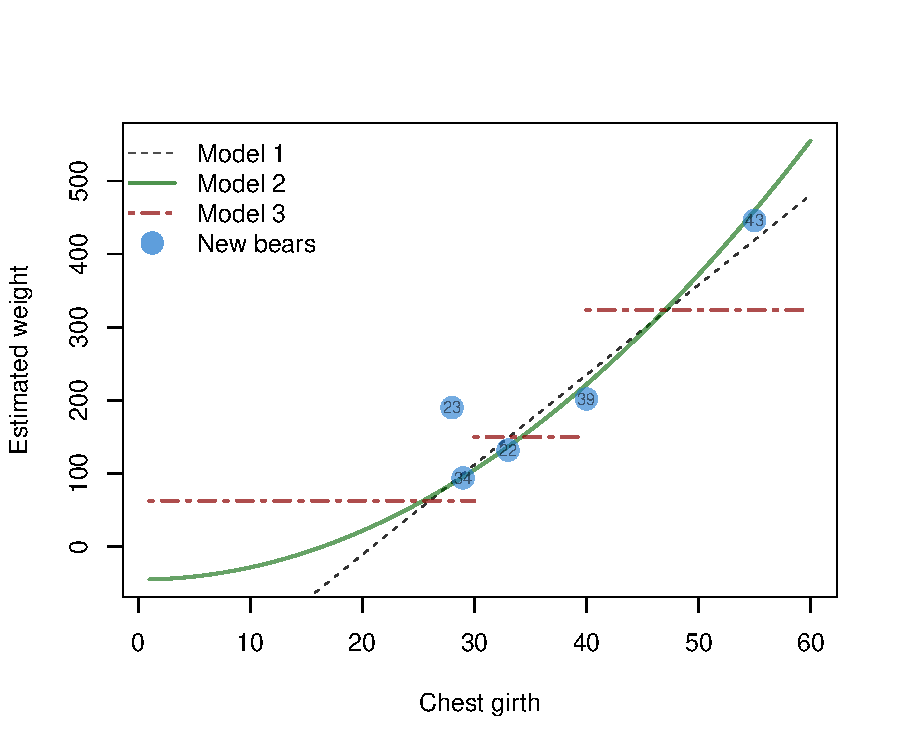
\includegraphics{exam2-009}
\end{center}
\begin{Schunk}
\begin{Sinput}
> ############# R CODE ######################
> plot(myseq, mod2(myseq), type="n",
+      xlab="Chest girth",
+      ylab="Estimated weight")
> lines(myseq, mod1(myseq), 
+       lty=2, lwd=1, col=adjustcolor("black", alpha.f=0.8))
> lines(myseq, mod2(myseq),
+       lty=1, lwd=2, col=adjustcolor("darkgreen", alpha.f=0.6))
> lines(1:30, rep(62.8125,30), lwd=2, lty=6,
+       col=adjustcolor("darkred", alpha.f=0.7))
> lines(30:40, rep(150,11), lwd=2, lty=6,
+       col=adjustcolor("darkred", alpha.f=0.7))
> lines(40:60, rep(323.4,21), lwd=2, lty=6,
+       col=adjustcolor("darkred", alpha.f=0.7))
> points(prob5$chest, prob5$weight, pch=16,
+        col=adjustcolor("dodgerblue3", alpha.f=0.6), cex=2)
> legend(x="topleft", lty=c(2,1,6, NA),
+        lwd=c(1,2,2, NA),
+        col=adjustcolor(c("black", "darkgreen", "darkred", "dodgerblue3"), alpha.f=0.7),
+        legend=c("Model 1", "Model 2", "Model 3", "New bears"),
+        pch=c(NA, NA, NA, 16), pt.cex=2, bty="n")
> text(prob5$chest, prob5$weight, labels=prob5$ID,
+      col=adjustcolor("black", alpha.f=0.5), cex=0.7)
\end{Sinput}
\end{Schunk}

\newpage
\subsection*{6. Model 4: Estimate and interpret the effects below:}
\addcontentsline{toc}{subsection}{Problem 6}





For the next few calculations, we'll use: $\hat{Y}=\beta_0 + \beta_1 X_1$  + \beta_2 X_2$  + \beta_3 X_3$ \\
where... \\
$\hat{Y}$ = estimated mean weight \\
$\beta_0$ = the estimate for the y-intercept \\
$X_1$ = age \\
$\beta_1$ = the regression coefficient for corresponding age\\
$X_2$ = gender=female \\
$\beta_2$ = the regression coefficient  for corresponding gender\\
$X_3$ = age*gender (if gender = female) \\
$\beta_3$ = the regression coefficient  for the interaction between female gender and age\\

\noindent Note that I intentionally left the parameter estimates for gender=MALE out of the above formula, given that they will always multiply to 0. \\

\noindent \textbf{a. Effect of a 6 month increase in age for Gender = M} \\
$\hat{Y}(age=6, gender=male) = \beta_0+ 6(5.64) + 0(13.77) + 0(6*-2.75*1) \\ - \beta_0+ 0(5.64) + 0(13.77) + 0(6*-2.75*1)$ \\
$\hat{Y}(age=6, gender=male) =  6(5.64) + 0(13.77) + 0(6*-2.75*1)$ \\
$\hat{Y}(age=6, gender=male) =  33.86$  \\

\fbox{
  \parbox{\textwidth}{
    \noindent Interpretation: Among males, holding constant other variables in our model, the mean effect of a 6 month increase in age on wieght is estimated to be 33.86 pounds.}
} \\



\noindent \textbf{b. Effect of a 6 month increase in age for Gender = F} \\
$\hat{Y}(age=6, gender=female) = \beta_0+ 6(5.64) + 1(13.77) + 1(6*-2.75*1) \\ 
- \beta_0+ 0(5.64) + 1(13.77) + 1(0*-2.75*1)$ \\

\noindent $\hat{Y} =  6(5.64) + 1(6*-2.75*1) $ \\
$\hat{Y(age=6, gender=female)} =   33.84 - 16.5 $ \\
$\hat{Y}(age=6, gender=female) =   17.34$ \\

\fbox{
  \parbox{\textwidth}{
    \noindent Interpretation: Among females, holding constant other variables in our model, the mean effect of a 6 month increase in age on wieght is estimated to be 17.34 pounds.}
} \\


\noindent \textbf{c. Comparing Males to Females at AGE = 24 months} \\
$\hat{Y}(age=24, gender=male) = \beta_0+ 24(5.64) + 0(13.77) + 0(24*-2.75*1) \\ 
$\hat{Y}(age=24, gender=female) = \beta_0+ 24(5.64) + 1(13.77) + 1(24*-2.75*1) \\ 

\noindent $\hat{Y}(age=24, gender=male) = 2.56 + 135.36 = 137.92  \\ 
$\hat{Y}(age=24, gender=female) = 2.56 + 135.36 + 13.77 - 66 = 85.69 \\ 
\noindent $\hat{Y}(age=24, gender=male) - \hat{Y}(females) = 52.3$ \\

\fbox{
  \parbox{\textwidth}{
    \noindent Interpretation: At 24 months old, holding constant other non-interacting variables in our model (chest girth), males are estimated to weight 52.3 pounds more than females on average.}
} \\



\noindent \textbf{d. Comparing Males to Females at AGE = 60 months} \\
$\hat{Y}(age=60, gender=male) =  2.56 + 60(5.64) + 0(13.77) + 0(60*-2.75*1) \\ 
$\hat{Y}(age=60, gender=female) = 2.56 + 60(5.64) + 1(13.77) + 1(60*-2.75*1) \\ 

\noindent $\hat{Y}(age=60, gender=male) = 2.56 + 338.4 = 340.96 \\ 
$\hat{Y}(age=60, gender=female) =  2.56 + 338.4 + 13.77 -165 = 189.73\\ 
\noindent $\hat{Y}(age=60, gender=male) - \hat{Y}(females) = 151.5 $ \\

\fbox{
  \parbox{\textwidth}{
    \noindent Interpretation: At 60 months old, holding constant other non-interacting variables in our model (chest girth), males are estimated to weight 151.5 pounds more than females on average.}
} \\

\begin{Schunk}
\begin{Sinput}
> ################ R CODE ########################
> prob6 <- function(age, gender){
+   2.55517023 + 
+     (5.64302247*age) + 
+     (gender*13.77721476) +
+     (age*gender*-2.75440159)
+ }
> prob6(age=20, gender=0) - prob6(age=14, gender=0) # PART A
\end{Sinput}
\begin{Soutput}
[1] 33.85813
\end{Soutput}
\begin{Sinput}
> prob6(age=30, gender=1) - prob6(age=24, gender=1) # PART B
\end{Sinput}
\begin{Soutput}
[1] 17.33173
\end{Soutput}
\begin{Sinput}
> prob6(age=24, gender=0) - prob6(age=24, gender=1) # PART C
\end{Sinput}
\begin{Soutput}
[1] 52.32842
\end{Soutput}
\begin{Sinput}
> prob6(age=60, gender=0) - prob6(age=60, gender=1) # PART D
\end{Sinput}
\begin{Soutput}
[1] 151.4869
\end{Soutput}
\end{Schunk}

\subsection*{Problem 6 visual}
\begin{center}
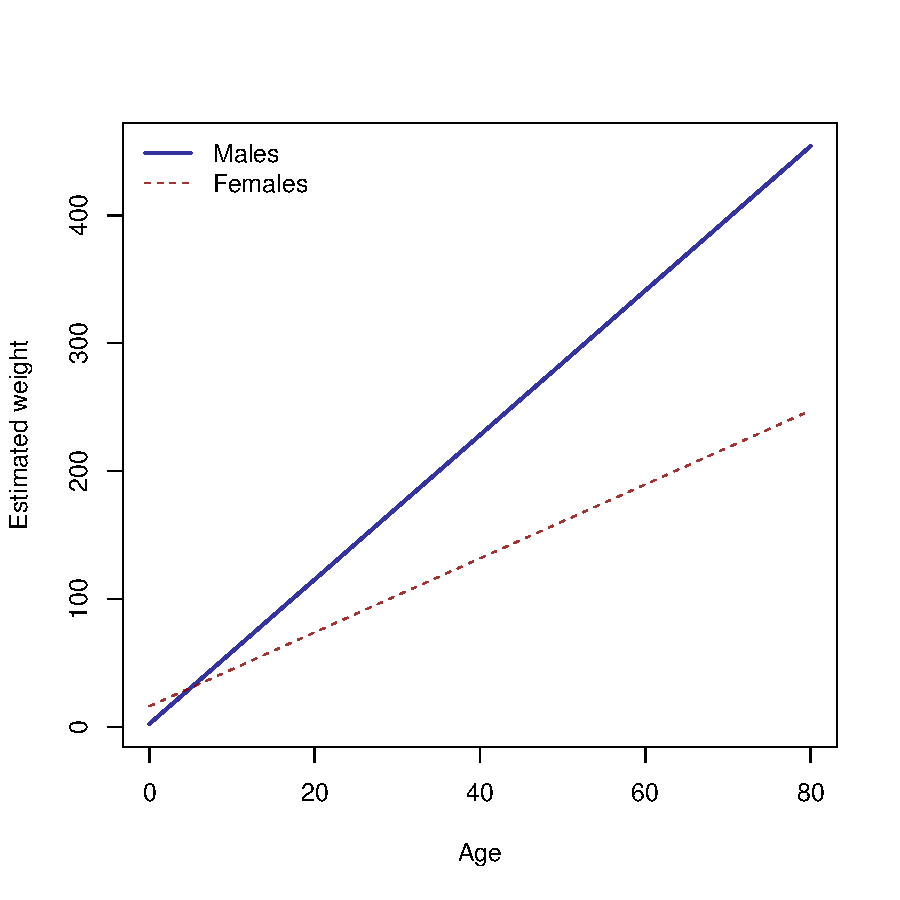
\includegraphics{exam2-012}
\end{center}
\begin{Schunk}
\begin{Sinput}
> #PROB 6 visual
> prob6seq <- seq(0,80,0.1)
> plot(prob6seq, prob6(age=prob6seq, gender=0), type="l",
+      xlab="Age", ylab="Estimated weight",
+      lty=1, lwd=2, col=adjustcolor("darkblue", alpha.f=0.8))
> lines(prob6seq, prob6(age=prob6seq, gender=1), type="l",
+       lty=2, lwd=1, col=adjustcolor("darkred", alpha.f=0.8))
> legend(x="topleft", lty=c(1,2), col=adjustcolor(c("darkblue", "darkred"), alpha.f=0.8),
+        lwd=c(2,1), legend=c("Males", "Females"), bty="n")
> 
\end{Sinput}
\end{Schunk}




\newpage
\subsection*{7. Model 6: Write the full estimated regression model for this model.}
As usual, we'll use the linear regression equation: \\
\addcontentsline{toc}{subsection}{Problem 7}


$\hat{Y}=\beta_0 + \beta_1 X_1$  + \beta_2 X_2$  + \beta_3 X_3$ \\
where... \\
$\hat{Y}$ = estimated mean weight \\
$\beta_0$ = the estimate for the y-intercept \\
$X_1$ = age\\
$\beta_1$ = the regression coefficient for age\\
$X_2$ = chest girth squared \\
$\beta_2$ = the regression coefficient for chest girth squared \\
$X_3$ = 1 if female, 0 if male (bivariate dummy) \\
$\beta_3$ = the regression coefficient  for gender\\
$X_4$ = age*gender (interaction term) \\
$\beta_4$ = the regression coefficient  for the interaction between female gender and age\\

$\hat{Y}(chest|age|gender) = -42.587 + chest*chest(0.127) + age(1.644) + gender(14.267) + age*gender(-1.00427258) \\ 

\noindent As before, for simplicity's sake, I have intentionally left out the zero terms for male gender and it's associated age interaction. \\

In R:\\
\begin{Schunk}
\begin{Sinput}
> mod6 <- function(chest, age, gender){
+   -42.58749126 + 
+     (chest*chest*0.12656138) +
+     (age*1.64485466) +
+     (gender*14.26653407) +
+     (age*gender*-1.00427258)
+ }
\end{Sinput}
\end{Schunk}




\newpage
\subsection*{8. Model 6: Estimate and interpret the following effects based upon this model using the following comparisons:} \\
\addcontentsline{toc}{subsection}{Problem 8}


\testbf{a. Increase in chest girth from 20 inches to 30 inches} \\

Since chest girth does not interact with any other variable in this model, we can simply give one estimate for the increase in chest girth for both males and females.  That said, for illustrative purposes (ie, to prove to myself), I use R to calculate male and female differently, arbitrarily setting age at 5 months. For the below example, I use 5 year-old females, though the increase would be the same for all ages and both sexes. \\

\noindent Females: $\hat{Y}(chest=30|age=5|gender=1) = -42.587 + 30*30(0.127) + 5(1.644) + 1(14.267) + 5*1(-1.00427258)$ \\ 
$\hat{Y}(chest=30|age=5|gender=1) = -42.59 + 114.3 + 8.2 + 14.27 - 5.02$ \\ 
$\hat{Y}(chest=30|age=5|gender=1) =  88.7872 $ \\ 

\noindent $\hat{Y}(chest=20|age=5|gender=1) = -42.587 + 20*20(0.127) + 5(1.644) + 1(14.267) + 5*1(-1.00427258)$ \\ 
$\hat{Y}(chest=20|age=5|gender=1) = -42.59 + 50.8 + 8.23 + 14.27 - 5.02$ \\ 
$\hat{Y}(chest=20|age=5|gender=1) = 25.50651 $ \\

\noindent Increase of (88.7872-25.50651) = 63.28069 pounds \\

\fbox{
  \parbox{\textwidth}{
    \noindent Interpretation: Holding constant the other variables in this model, an increase in chest girth from 20 to 30 inches is estimated to portend a 63.5 pound mean increase in weight.
  }
}


\begin{Schunk}
\begin{Sinput}
> ############ R CODE ########################
> mod6(chest=30, age=5, gender=1) - mod6(chest=20, age=5, gender=1) #Females
\end{Sinput}
\begin{Soutput}
[1] 63.28069
\end{Soutput}
\begin{Sinput}
> mod6(chest=30, age=5, gender=0) - mod6(chest=20, age=5, gender=0) #Males
\end{Sinput}
\begin{Soutput}
[1] 63.28069
\end{Soutput}
\end{Schunk}


\testbf{b. Increase in chest girth from 40 inches to 50 inches} \\
For the below example calculation, I used 5 year-old males.  Given that chest girth does not interact with other variables, we would find the same difference for any age and both sexes.

\noindent $\hat{Y}(chest=40|age=5|gender=0) = -42.587 + 40*40(0.127) + 5(1.644) $ \\ 
$\hat{Y}(chest=30|age=5|gender=1) = -42.587 + 203.2+ 8.225 $ \\ 
$\hat{Y}(chest=30|age=5|gender=1) = 168.135 $ \\ 

\noindent $\hat{Y}(chest=50|age=5|gender=0) = -42.587 + 50*50(0.127) + 5(1.644) $ \\ 
$\hat{Y}(chest=30|age=5|gender=1) = -42.587 + 317.5 + 8.225 $ \\ 
$\hat{Y}(chest=30|age=5|gender=1) = 282.0402 $ \\ 

\noindent Increase of (282.04-168.14) = 113.905 pounds\\ 

\fbox{
  \parbox{\textwidth}{
    \noindent Interpretation: Holding constant the other variables in this model, an increase in chest girth from 30 to 40 inches is estimated to portend a 113.91 pound mean increase in weight.
  }
}


\begin{Schunk}
\begin{Sinput}
> ############ R CODE ########################
> mod6(chest=50, age=5, gender=0) - mod6(chest=40, age=5, gender=0) 
\end{Sinput}
\begin{Soutput}
[1] 113.9052
\end{Soutput}
\end{Schunk}

\noindent \textbf{c. Effect of a 6 month increase in age for Gender = M.} \\
\noindent $\hat{Y}(chest=40|age=6|gender=0) = -42.587 + (40*40*0.127) + (6*1.644) $ \\ 
$\hat{Y}(chest=40|age=6|gender=0) =  169.7798 $ \\ 

\noindent $\hat{Y}(chest=40|age=6|gender=0) = -42.587 + (40*40*0.127) + (0*1.644) $ \\ 
$\hat{Y}(chest=40|age=6|gender=0) =  160.613$ \\ 

\noindent Increase of (169.78-160.61) = 9.869128 pounds \\

\fbox{
  \parbox{\textwidth}{
    \noindent Interpretation: For males, holding constant the other non-interacting variables in this model, an 6 month increase in age is estimated to portend a 9.87 pound mean increase in weight.
  }
}

\begin{Schunk}
\begin{Sinput}
> ############ R CODE ########################
> mod6(chest=40, age=6, gender=0) -mod6(chest=40, age=0, gender=0)
\end{Sinput}
\begin{Soutput}
[1] 9.869128
\end{Soutput}
\end{Schunk}


\noindent \textbf{d. Effect of a 6 month increase in age for Gender = F.} \\
\noindent $\hat{Y}(chest=40|age=6|gender=1) = -42.587 + (40*40*0.127) + (6*1.644) + (1*14.267) + (6*1*-1.00427258)$ \\ 
$\hat{Y}(chest=40|age=6|gender=1) = 178.0207 $ \\ 

\noindent $\hat{Y}(chest=40|age=0|gender=1) = -42.587 + (40*40*0.127) + (1*14.267) $ \\ 
$\hat{Y}(chest=40|age=6|gender=1) = 174.88 $ \\ 

\noindent Increase of (178.02-174.88) = 3.84 pounds \\

\fbox{
  \parbox{\textwidth}{
    \noindent Interpretation: For females, holding constant the other non-interacting variables in this model, an 6 month increase in age is estimated to portend a 3.84 pound mean increase in weight.
  }
}

\begin{Schunk}
\begin{Sinput}
> ############ R CODE ########################
> mod6(chest=40, age=6, gender=1) -mod6(chest=40, age=0, gender=1)
\end{Sinput}
\begin{Soutput}
[1] 3.843492
\end{Soutput}
\end{Schunk}


\noindent \textbf{e. Comparing Males to Females at AGE = 24 months} \\

\noindent Male: $\hat{Y}(chest=40|age=24|gender=0) = -42.587 + (40*40*0.127) + (24*1.644)$ \\ 
$\hat{Y}(chest=40|age=24|gender=1) = 200.069 $ \\ 

\noindent Female: $\hat{Y}(chest=40|age=24|gender=1) = -42.587 + (40*40*0.127) + (24*1.644) + (1*14.267) + (24*1*-1.00427258)$ \\ 
$\hat{Y}(chest=40|age=24|gender=1) = 190.2335 $ \\ 

\noindent Increase of (200.07-190.23) = 9.836008 pounds \\

\fbox{
  \parbox{\textwidth}{
    \noindent Interpretation: On average (or holding other non-interacting variables constant), at 24 months of age, males are expected to weigh 9.84 pounds more than females.}
}

\begin{Schunk}
\begin{Sinput}
> ############ R CODE ########################
> mod6(chest=40, age=24, gender=0) -mod6(chest=40, age=24, gender=1)
\end{Sinput}
\begin{Soutput}
[1] 9.836008
\end{Soutput}
\end{Schunk}

\noindent \textbf{f. Comparing Males to Females at AGE = 60 months}\\

\noindent Male: $\hat{Y}(chest=40|age=60|gender=0) = -42.587 + (40*40*0.127) + (60*1.644)$ \\ 
$\hat{Y}(chest=40|age=24|gender=1) = 259.25 $ \\ 

\noindent Female: $\hat{Y}(chest=40|age=60|gender=1) = -42.587 + (40*40*0.127) + (60*1.644) + (1*14.267) + (60*1*-1.00427258)$ \\ 
$\hat{Y}(chest=40|age=24|gender=1) = 213.26 $ \\ 

\noindent Increase of (259.25-213.26) = 45.99 pounds \\


\fbox{
  \parbox{\textwidth}{
    \noindent Interpretation: On average (or holding other non-interacting variables constant), at 60 months of age, males are expected to weigh 45.99 pounds more than females.}
}





\begin{Schunk}
\begin{Sinput}
> ############ R CODE ########################
> mod6(chest=40, age=60, gender=0) -mod6(chest=40, age=60, gender=1)
\end{Sinput}
\begin{Soutput}
[1] 45.98982
\end{Soutput}
\end{Schunk}

\newpage
\subsection*{9. Using models 4 and 6: For the 5 NEW bears below (not used in our model), predict the weight of the bear and provide the residual error using these two models.}\\
\addcontentsline{toc}{subsection}{Problem 9}



% latex table generated in R 3.0.2 by xtable 1.7-1 package
% Thu Apr 17 19:08:53 2014
\begin{table}[ht]
\centering
\begin{tabular}{rlrrlrrrrrr}
  \hline
 & ID & weight & chest & size & age & gender & model4 & model4error & model6 & model6error \\ 
  \hline
1 & 22 & 132.00 & 33.00 & medium & 81.00 & 1.00 & 250.31 & -118.31 & 161.39 & -29.39 \\ 
  2 & 23 & 190.00 & 28.00 & small & 21.00 & 0.00 & 121.06 & 68.94 & 91.18 & 98.82 \\ 
  3 & 34 & 94.00 & 29.00 & small & 10.00 & 0.00 & 58.99 & 35.01 & 80.30 & 13.70 \\ 
  4 & 39 & 202.00 & 40.00 & large & 58.00 & 1.00 & 183.87 & 18.13 & 211.33 & -9.33 \\ 
  5 & 43 & 446.00 & 55.00 & large & 70.00 & 0.00 & 397.57 & 48.43 & 455.40 & -9.40 \\ 
   \hline
\end{tabular}
\end{table}

\begin{Schunk}
\begin{Sinput}
> prob9 <- prob5[c(1,2,3,8)]
> prob9$age <- c(81, 21, 10, 58, 70)
> prob9$gender <- c(1,0,0,1,0)
> mod4 <- prob6 #renames function for model 4
> prob9$model4 <- mod4(age=prob9$age, gender=prob9$gender)
> prob9$model4error <- prob9$weight - prob9$model4
> prob9$model6 <- mod6(chest= prob9$chest, age=prob9$age, gender=prob9$gender)
> prob9$model6error <- prob9$weight - prob9$model6
\end{Sinput}
\end{Schunk}

\newpage

\section*{Part 2: NHANES Data (50 points)}
\addcontentsline{toc}{section}{Part 2}

\subsection*{10. The following is the SAS output for a simple logistic regression model evaluating the effect of age on the risk of high blood pressure (HBP). The probability of HBP = YES is modeled.}
\addcontentsline{toc}{subsection}{Problem 10}

For this section, we'll be using the following formula: \\

\noindent $ log(\frac{(p(X)}{1-p(X)}) = \beta_0+\beta_1 X_1 \pm e $ \\

where...\\

\noindent $ p(X)$ = the probability of event (HBP=yes) \\
$ log(\frac{(p(X)}{1-p(X)})$ = the log of the odds ratio \\
$ \beta_0 $ = the y-intercept \\
$ X_1$ = age\\
$ \beta_1$ = the parameter estimate / regression coefficient for age\\
$ e $ = standard error for the estimate(s)\\




\noindent \textbf{a. Provide the estimated regression model.} \\

\noindent $ log(\frac{(p(X)}{1-p(X)}) = \beta_0+\beta_1 X_1 \pm e $\\

\noindent $ log(\frac{(p(X)}{1-p(X)}) = -4.7551 + (0.0646*age)$ \\


\noindent \textbf{b. Find the odds ratio of high blood pressure for a 1-year increase in age and the associated 95\% confidence interval.} \\

\noindent $ log(odds ratio) = 0.0646 $\\
odds ratio = exp(0.0646)  \\
1.066732 \\

\noindent 95\% C.I. = \\
exp(0.646)-exp(0.00241) [low] \\
exp(0.646)+exp(0.00241) [high]\\
0.905-2.910 \\



\noindent \textbf{c. Find the odds ratio of high blood pressure for a 10-year increase in age.} \\

\noindent $ log(odds ratio) = 0.0646*10 \\
exp(0.0646*10) \\
1.908

%%%%%%%%%%%%%%%%%%%%%%%%%%%%%%%%%%%%%%%%%%%%%%%%%%%%%%%%%%%%%%%%
\subsection*{11. The interaction effect between gender (SEX) and age was considered in a multiple logistic regression model.  The output is provided below.  The probability of HBP = Yes is modeled.}
\addcontentsline{toc}{subsection}{Problem 11}

\noindent \textbf{a. State the fitted (estimated) regression model.} \\
\noindent $ log(\frac{(p(X)}{1-p(X)}) = \beta_0+\beta_1 X_1 +\beta_2 X_2 +\beta_3 X_3\pm e $ \\

where...\\

\noindent $ p(X)$ = the probability of event (HBP=yes) \\
$ log(\frac{(p(X)}{1-p(X)})$ = the log of the odds ratio \\
$ \beta_0 $ = the y-intercept \\
$ X_1$ = sex (1 if male, 0 if female)\\
$ \beta_1$ = the parameter estimate / regression coefficient for sex\\
$ X_2$ = age\\
$ \beta_2$ = the parameter estimate / regression coefficient for age\\
$ X_3$ = age times sex (interaction term) \\
$ \beta_3$ = the parameter estimate / regression coefficient for the interaction of age and sex\\
$ e $ = standard error for the estimate(s)\\

If we fill it in, we get... \\

\noindent $ log(\frac{(p(X)}{1-p(X)}) = -5.0842 + (sex*0.6890) + (age*0.0702) + (age*sex*-0.0118)$\\

\noindent \pm SE:$ (\pm 0.2190 \pm 0.3111 \pm 0.00338 \pm 0.00482 $ \\

In R, it looks like:
\begin{Schunk}
\begin{Sinput}
> prob11logOdds<- function(sex, age){
+     -5.0842 + 
+     (sex*0.6890) +
+     (age*0.0702) +
+     (age*sex*-0.0118)
+ }
> prob11odds<- function(sex, age){
+   logOdds <- 
+     -5.0842 + 
+     (sex*0.6890) +
+     (age*0.0702) +
+     (age*sex*-0.0118)
+   exp(logOdds)
+ }
\end{Sinput}
\end{Schunk}


\newpage
\noindent \textbf{b. Calculate the odds ratio of high blood pressure comparing males to females for individuals age 40.} \\

\noindent $ log(\frac{(p(X)}{1-p(X)}) = -5.0842 + (sex*0.6890) + (age*0.0702) + (age*sex*-0.0118)$\\

\noindent MALES $ log(\frac{(p(X)}{1-p(X)}) = -5.0842 + (1*0.6890) + (40*0.0702) + (40*1*-0.0118)$\\
Males log(odds): -2.0592 \\
Male odds: 0.127556\\

\noindent FEMALES $ log(\frac{(p(X)}{1-p(X)}) = -5.0842 + (0*0.6890) + (40*0.0702) + (40*0*-0.0118)$\\
Females log(odds): -2.2762 \\
Female odds: 0.1026736 \\

\noindent Odds ratio (0.128/0.103) = 1.242 (males to females at age 40) \\

\fbox{
  \parbox{\textwidth}{
    \noindent Interpretation: Among 40 year-olds, males have 1.24 greater odds for HBP than females.}
} \\

\begin{Schunk}
\begin{Sinput}
> ############# R CODE #########################
> prob11odds(sex=1, age=40) / prob11odds(sex=0, age=40)
\end{Sinput}
\begin{Soutput}
[1] 1.242344
\end{Soutput}
\end{Schunk}



\noindent \textbf{c. Calculate the odds ratio of highblood pressure comparing males to females for individuals age 80.} \\

\noindent $ log(\frac{(p(X)}{1-p(X)}) = -5.0842 + (sex*0.6890) + (age*0.0702) + (age*sex*-0.0118)$\\

\noindent MALES $ log(\frac{(p(X)}{1-p(X)}) = -5.0842 + (1*0.6890) + (80*0.0702) + (80*1*-0.0118)$\\
Males log(odds): 0.2768 \\
Male odds: 1.318903 \\


\noindent FEMALES $ log(\frac{(p(X)}{1-p(X)}) = -5.0842 + (0*0.6890) + (80*0.0702) + (80*0*-0.0118)$\\
Females log(odds): 0.5318 \\
Female odds: 1.701993


\noindent Odds ratio (1.318903/1.701993) = 0.7749168 (males to females at age 80) \\

\fbox{
  \parbox{\textwidth}{
    \noindent Interpretation: Among 80 year-olds, males are 0.77 times as likely to have HBP than females. In other words, females have 1.29 the odds of HBP as males (at age 80).}
} \\

\begin{Schunk}
\begin{Sinput}
> ############# R CODE #########################
> prob11odds(sex=1, age=80) / prob11odds(sex=0, age=80)
\end{Sinput}
\begin{Soutput}
[1] 0.7749165
\end{Soutput}
\end{Schunk}

\noindent \textbf{d. Calculate the odds ratio of high blood pressure for a 10-year change in age among males.  } \\

\noindent $ log(\frac{(p(X)}{1-p(X)}) = -5.0842 + (sex*0.6890) + (age*0.0702) + (age*sex*-0.0118)$\\
\noindent $ log(\frac{(p(X)}{1-p(X)}) =  (10*0.0702) + (10*1*-0.0118)$\\
\noindent log(odds ratio): 0.584 \\
\noindent odds ratio: 1.793197\\

\begin{Schunk}
\begin{Sinput}
> ############# R CODE #########################
> prob11odds(sex=1, age=80) / prob11odds(sex=1, age=70) #note: the two are equivalent
\end{Sinput}
\begin{Soutput}
[1] 1.793197
\end{Soutput}
\begin{Sinput}
> prob11odds(sex=1, age=70) / prob11odds(sex=1, age=60)
\end{Sinput}
\begin{Soutput}
[1] 1.793197
\end{Soutput}
\begin{Sinput}
> 
\end{Sinput}
\end{Schunk}

\fbox{
  \parbox{\textwidth}{
    \noindent Interpretation: Among men, a 10 year increase in age is associated with an increase of 1.79 in the odds of HBP. }
} \\

\noindent \textbf{e. Calculate the predicted probability of high blood pressure for a male of age 40 and again for a female of age 40.} \\

\noindent In part B, we already calculated the odds of HBP for both men and women at age 40:\\
Male odds: 0.127556\\
Female odds: 0.1026736 \\

\noindent To convert odds to probability, all we have to do is divide the odds by 1+the odds: \\
Male probability: 0.127556 / (1+0.127556) = 0.1131261 \\
Female probability: 0.1026736 / (1+0.1026736) = 0.09311332  \\

We could also write an R function to convert log(odds) to probability.\\
\begin{Schunk}
\begin{Sinput}
> ############# R CODE #########################
> prob11probability<- function(sex, age){
+     odds <-
+       exp(
+       -5.0842 + 
+     (sex*0.6890) +
+     (age*0.0702) +
+     (age*sex*-0.0118))
+     odds / (1+odds)    
+ }
\end{Sinput}
\end{Schunk}


\begin{Schunk}
\begin{Sinput}
> ############# R CODE #########################
> prob11probability(sex=1, age=40) #male
\end{Sinput}
\begin{Soutput}
[1] 0.1131261
\end{Soutput}
\begin{Sinput}
> prob11probability(sex=0, age=40) #female
\end{Sinput}
\begin{Soutput}
[1] 0.09311334
\end{Soutput}
\begin{Sinput}
> 
\end{Sinput}
\end{Schunk}


\fbox{
  \parbox{\textwidth}{
    \noindent Interpretation: 40 year-old men have an 0.113 probability of HBP.  40 year-old women have a 0.093 probability of HBP.}
} \\


\newpage
\subsection*{12. The following is the SAS output for a simple logistic regression model evaluating the effect of BMI group on the risk of high blood pressure (HBP).  The probability of HBP = Yes is modeled.}
\addcontentsline{toc}{subsection}{Problem 12}


\noindent \textbf{a. Briefly discuss the conclusions for this predictor.  Include interpretations of any significant odds ratios.} \\

I appears that as weight increases, so do the odds of HBP.  Obese individuals have significantly greater odds for HBP than do those in the "normal" weight category (OR: 1.227, 95\% C.I. = 1.054-1.429 ).  And though the odds of HBP among overweight is not \emph{significantly} greater than it is among those at normal weight (at the p = 0.05 significance level), it is still directionally indicative of a likely risk factor.  

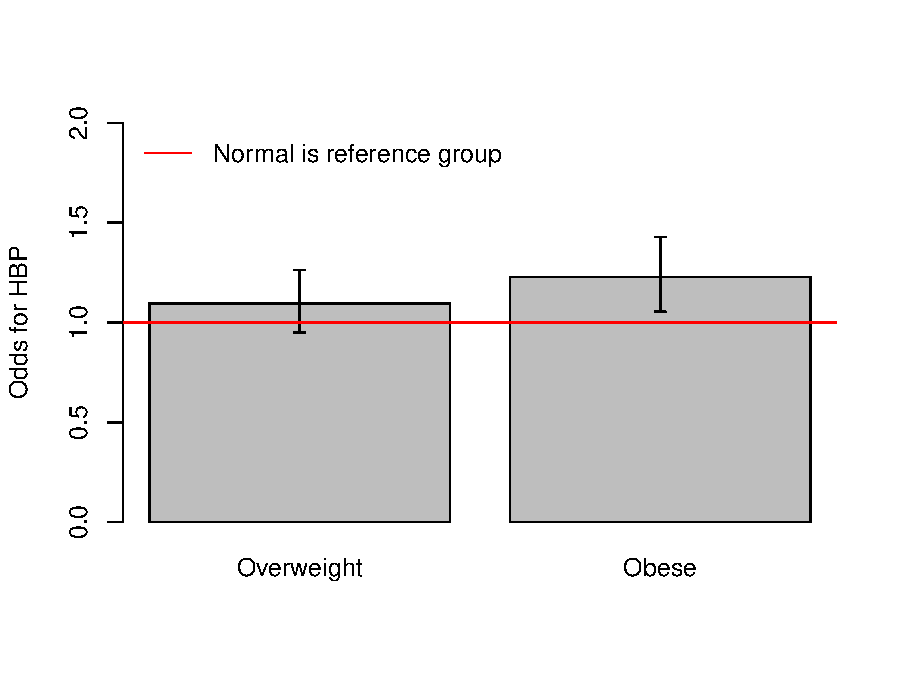
\includegraphics{exam2-030}

\begin{Schunk}
\begin{Sinput}
> ############ R CODE ########################
> library(Hmisc)
> OR <- c(1, exp(0.0907), exp(0.2049))
> low <- c(1, exp(0.0907 - (1.96*0.0726)), exp(0.2049 - (1.96*0.0777)))
> high <- c(1, exp(0.0907 + (1.96*0.0726)), exp(0.2049 + (1.96*0.0777)))
> mybp <- barplot(OR[2:3], ylim=c(0,2),
+                 names.arg=c("Overweight", "Obese"), ylab="Odds for HBP")
> errbar(x=mybp[,1], y= OR[2:3], 
+        yplus= high[2:3],
+        ymin= low[2:3],
+        add=T, xlab="", pch=".")
> legend(x="topleft", lty=1, col="red", legend="Normal is reference group",
+        bty="n", border=FALSE)
> abline(h=1, col="red")
\end{Sinput}
\end{Schunk}



\noindent \textbf{b. Calculate the predicted probability of high blood pressure in each group.} \\
Probability is simply the odds divided by 1 + odds, so:\\

\noindent prob(HBP|weight = normal) = exp(-0.9256) / (1+exp(-0.9256)) = 0.2838182\\
\noindent prob(HBP|weight = overweight) = exp(0.0907) / (1+exp(0.0907)) = 0.5226595\\
\noindent prob(HBP|weight = obese) = exp(0.2049) / (1+exp(0.2049)) = 0.5510465\\


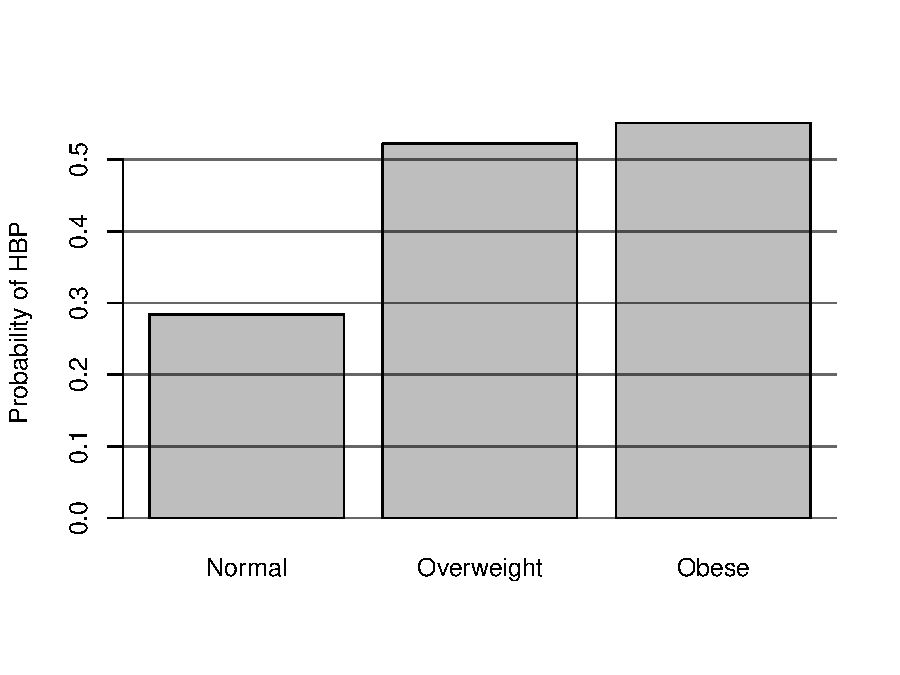
\includegraphics{exam2-033}

\begin{Schunk}
\begin{Sinput}
> barplot(probs, names.arg=c("Normal", "Overweight", "Obese"),
+         ylab="Probability of HBP")
> abline(h=seq(0,.5, .1), col=adjustcolor("black", alpha.f=0.6))
\end{Sinput}
\end{Schunk}


\newpage
\subsection*{13. A full logistic regression model is performed.  The output is provided as needed.}
\addcontentsline{toc}{subsection}{Problem 13}

\noindent \textbf{a. Consider the "Class level information" output from SAS. Explain clearly what this output indicates about the current regression model.} \\
The "Class Level Information" here indicates both the potential levels for each variable, and more importantly, which level will be used as the "reference" for relative statistics (the calculation of odds, odds ratios, etc.).  In this case, the reference group is female, white and normal. \\

Given that it's beyond dichotomous, "bmigroup" deserves special attention.  For this variable, "dummies" had to be created so as to calculate $\_beta$ estimates when going from the reference ("normal") to both overweight and obese. This is a common technique for dealing with multi-level categorical variables, and SAS handles this kind of information in its generalized linear models approach (or, alternatively, by manually creating dummy variables in a normal linear regression). \\


\noindent \textbf{b. Using the output on the last page, correctly interpret all signficant odds ratios presented.} \\

\noindent Among females, holding all other variables in the model constant, the odds of HBP among the normal are 0.612 those of the obese, with a 95\% confidence interval of 0.515 to 0.728. This association is statistically significant at the p=0.05 level. \\

\noindent Among females, holding all other variables in the model constant, the odds of HBP among the normal are 0.852 those of the obese, with a 95\% confidence interval of 0.727 to 0.998. This association is statistically significant at the p=0.05 level. \\

\noindent Among females, holding all other variables in the model constant, the odds of HBP among the obese are 1.391 those of the overweight, with a 95\% confidence interval of 1.180 to 1.640. This association is statistically significant at the p=0.05 level.  \\

\noindent Among females, holding all other non-interacting variables in the model constant (race, BMIgroup), the odds of HBP among black people are 1.562 those of the white, with a 95\% confidence interval of 1.339 to 1.821. This association is statistically significant at the p=0.05 level.\\

\noindent Among females, holding all other variables in the model constant, an increase of 50 in TCP units is associated with an increased odds of HBP of 13\%, with a 95\% confidence interval of 4.7\% to 21.9\%. This association is statistically significant at the p=0.05 level.\\

\noindent Among 40 year-olds , holding all other (non-interacting) variables in the model constant, the odds of HBP among females are 0.758 those of males, with a 95\% confidence interval of 0.585 to 0.983. This association is statistically significant at the p=0.05 level.\\

\noindent Among 50 year-olds, holding all other variables in the model constant, the odds of HBP among females are 0.846 those of males, with a 95\% confidence interval of 0.704 to 1.017. This association is not statistically significant at the p=0.05 level.\\

\noindent Among 60 year-olds, holding all other variables in the model constant, the odds of HBP among females are 0.944 those of males, with a 95\% confidence interval of 0.823 to 1.084. This association is not statistically significant at the p=0.05 level.\\

\noindent Among 70 year-olds, holding all other variables in the model constant, the odds of HBP among females are 1.054 those of males, with a 95\% confidence interval of 0.907 to 1.225. This association is not statistically significant at the p=0.05 level. \\

\noindent Among 80 year-olds, holding all other variables in the model constant, the odds of HBP among females are 1.177 those of males, with a 95\% confidence interval of 0.952 to 1.454. This association is not statistically significant at the p=0.05 level. \\

\noindent Among females, holding all other variables in the model constant, an increase of 10 age units is associated with a doubling of the odds of HBP (odds ratio: 2.096, 95\% C.I. = 1.955 to 2.247). This association is statistically significant at the p=0.05 level.\\

\noindent Among males, holding all other variables in the model constant, a 10 unit increase in age is associated with 1.878 the odds of HBP (ie, an 88\% increase), with a 95\% confidence interval of 1.752 to 2.012). This association is statistically significant at the p=0.05 level. \\



\end{document}
